% Options for packages loaded elsewhere
\PassOptionsToPackage{unicode}{hyperref}
\PassOptionsToPackage{hyphens}{url}
%
\documentclass[
]{book}
\usepackage{amsmath,amssymb}
\usepackage{lmodern}
\usepackage{iftex}
\ifPDFTeX
  \usepackage[T1]{fontenc}
  \usepackage[utf8]{inputenc}
  \usepackage{textcomp} % provide euro and other symbols
\else % if luatex or xetex
  \usepackage{unicode-math}
  \defaultfontfeatures{Scale=MatchLowercase}
  \defaultfontfeatures[\rmfamily]{Ligatures=TeX,Scale=1}
\fi
% Use upquote if available, for straight quotes in verbatim environments
\IfFileExists{upquote.sty}{\usepackage{upquote}}{}
\IfFileExists{microtype.sty}{% use microtype if available
  \usepackage[]{microtype}
  \UseMicrotypeSet[protrusion]{basicmath} % disable protrusion for tt fonts
}{}
\makeatletter
\@ifundefined{KOMAClassName}{% if non-KOMA class
  \IfFileExists{parskip.sty}{%
    \usepackage{parskip}
  }{% else
    \setlength{\parindent}{0pt}
    \setlength{\parskip}{6pt plus 2pt minus 1pt}}
}{% if KOMA class
  \KOMAoptions{parskip=half}}
\makeatother
\usepackage{xcolor}
\usepackage{color}
\usepackage{fancyvrb}
\newcommand{\VerbBar}{|}
\newcommand{\VERB}{\Verb[commandchars=\\\{\}]}
\DefineVerbatimEnvironment{Highlighting}{Verbatim}{commandchars=\\\{\}}
% Add ',fontsize=\small' for more characters per line
\usepackage{framed}
\definecolor{shadecolor}{RGB}{248,248,248}
\newenvironment{Shaded}{\begin{snugshade}}{\end{snugshade}}
\newcommand{\AlertTok}[1]{\textcolor[rgb]{0.94,0.16,0.16}{#1}}
\newcommand{\AnnotationTok}[1]{\textcolor[rgb]{0.56,0.35,0.01}{\textbf{\textit{#1}}}}
\newcommand{\AttributeTok}[1]{\textcolor[rgb]{0.77,0.63,0.00}{#1}}
\newcommand{\BaseNTok}[1]{\textcolor[rgb]{0.00,0.00,0.81}{#1}}
\newcommand{\BuiltInTok}[1]{#1}
\newcommand{\CharTok}[1]{\textcolor[rgb]{0.31,0.60,0.02}{#1}}
\newcommand{\CommentTok}[1]{\textcolor[rgb]{0.56,0.35,0.01}{\textit{#1}}}
\newcommand{\CommentVarTok}[1]{\textcolor[rgb]{0.56,0.35,0.01}{\textbf{\textit{#1}}}}
\newcommand{\ConstantTok}[1]{\textcolor[rgb]{0.00,0.00,0.00}{#1}}
\newcommand{\ControlFlowTok}[1]{\textcolor[rgb]{0.13,0.29,0.53}{\textbf{#1}}}
\newcommand{\DataTypeTok}[1]{\textcolor[rgb]{0.13,0.29,0.53}{#1}}
\newcommand{\DecValTok}[1]{\textcolor[rgb]{0.00,0.00,0.81}{#1}}
\newcommand{\DocumentationTok}[1]{\textcolor[rgb]{0.56,0.35,0.01}{\textbf{\textit{#1}}}}
\newcommand{\ErrorTok}[1]{\textcolor[rgb]{0.64,0.00,0.00}{\textbf{#1}}}
\newcommand{\ExtensionTok}[1]{#1}
\newcommand{\FloatTok}[1]{\textcolor[rgb]{0.00,0.00,0.81}{#1}}
\newcommand{\FunctionTok}[1]{\textcolor[rgb]{0.00,0.00,0.00}{#1}}
\newcommand{\ImportTok}[1]{#1}
\newcommand{\InformationTok}[1]{\textcolor[rgb]{0.56,0.35,0.01}{\textbf{\textit{#1}}}}
\newcommand{\KeywordTok}[1]{\textcolor[rgb]{0.13,0.29,0.53}{\textbf{#1}}}
\newcommand{\NormalTok}[1]{#1}
\newcommand{\OperatorTok}[1]{\textcolor[rgb]{0.81,0.36,0.00}{\textbf{#1}}}
\newcommand{\OtherTok}[1]{\textcolor[rgb]{0.56,0.35,0.01}{#1}}
\newcommand{\PreprocessorTok}[1]{\textcolor[rgb]{0.56,0.35,0.01}{\textit{#1}}}
\newcommand{\RegionMarkerTok}[1]{#1}
\newcommand{\SpecialCharTok}[1]{\textcolor[rgb]{0.00,0.00,0.00}{#1}}
\newcommand{\SpecialStringTok}[1]{\textcolor[rgb]{0.31,0.60,0.02}{#1}}
\newcommand{\StringTok}[1]{\textcolor[rgb]{0.31,0.60,0.02}{#1}}
\newcommand{\VariableTok}[1]{\textcolor[rgb]{0.00,0.00,0.00}{#1}}
\newcommand{\VerbatimStringTok}[1]{\textcolor[rgb]{0.31,0.60,0.02}{#1}}
\newcommand{\WarningTok}[1]{\textcolor[rgb]{0.56,0.35,0.01}{\textbf{\textit{#1}}}}
\usepackage{longtable,booktabs,array}
\usepackage{calc} % for calculating minipage widths
% Correct order of tables after \paragraph or \subparagraph
\usepackage{etoolbox}
\makeatletter
\patchcmd\longtable{\par}{\if@noskipsec\mbox{}\fi\par}{}{}
\makeatother
% Allow footnotes in longtable head/foot
\IfFileExists{footnotehyper.sty}{\usepackage{footnotehyper}}{\usepackage{footnote}}
\makesavenoteenv{longtable}
\usepackage{graphicx}
\makeatletter
\def\maxwidth{\ifdim\Gin@nat@width>\linewidth\linewidth\else\Gin@nat@width\fi}
\def\maxheight{\ifdim\Gin@nat@height>\textheight\textheight\else\Gin@nat@height\fi}
\makeatother
% Scale images if necessary, so that they will not overflow the page
% margins by default, and it is still possible to overwrite the defaults
% using explicit options in \includegraphics[width, height, ...]{}
\setkeys{Gin}{width=\maxwidth,height=\maxheight,keepaspectratio}
% Set default figure placement to htbp
\makeatletter
\def\fps@figure{htbp}
\makeatother
\setlength{\emergencystretch}{3em} % prevent overfull lines
\providecommand{\tightlist}{%
  \setlength{\itemsep}{0pt}\setlength{\parskip}{0pt}}
\setcounter{secnumdepth}{5}
\usepackage{booktabs}
\ifLuaTeX
  \usepackage{selnolig}  % disable illegal ligatures
\fi
\usepackage[]{natbib}
\bibliographystyle{plainnat}
\IfFileExists{bookmark.sty}{\usepackage{bookmark}}{\usepackage{hyperref}}
\IfFileExists{xurl.sty}{\usepackage{xurl}}{} % add URL line breaks if available
\urlstyle{same} % disable monospaced font for URLs
\hypersetup{
  pdftitle={Soil and Vegetation Survey of the Willow National Petroleum Reserve-Alaska},
  pdfauthor={Gabriel Benitez, Nathan Roe, and Blaine Spellman},
  hidelinks,
  pdfcreator={LaTeX via pandoc}}

\title{Soil and Vegetation Survey of the Willow National Petroleum Reserve-Alaska}
\author{Gabriel Benitez, Nathan Roe, and Blaine Spellman}
\date{2024-10-17}

\usepackage{amsthm}
\newtheorem{theorem}{Theorem}[chapter]
\newtheorem{lemma}{Lemma}[chapter]
\newtheorem{corollary}{Corollary}[chapter]
\newtheorem{proposition}{Proposition}[chapter]
\newtheorem{conjecture}{Conjecture}[chapter]
\theoremstyle{definition}
\newtheorem{definition}{Definition}[chapter]
\theoremstyle{definition}
\newtheorem{example}{Example}[chapter]
\theoremstyle{definition}
\newtheorem{exercise}{Exercise}[chapter]
\theoremstyle{definition}
\newtheorem{hypothesis}{Hypothesis}[chapter]
\theoremstyle{remark}
\newtheorem*{remark}{Remark}
\newtheorem*{solution}{Solution}
\begin{document}
\maketitle

{
\setcounter{tocdepth}{1}
\tableofcontents
}
\hypertarget{interactive-project-map}{%
\chapter{Interactive Project Map}\label{interactive-project-map}}

\hypertarget{introduction}{%
\section{Introduction}\label{introduction}}

The survey area within the National Petroleum Reserve-Alaska (NPR-A) is in the Arctic Coastal Plain of the North Slope of Alaska, approximately 90 miles (145 km) west of Prudhoe Bay. These lands were originally inhabited by various Alaska Native groups, including the Inupiat people for thousands of years. In 1923, President Warren G. Harding established the Naval Petroleum Reserve No.4 (NPR-4) through an executive order, which brought this area under federal ownership without consultation or compensation to the Alaska Native peoples. In 1976, the Naval Petroleum Reserves Production Act renamed the area to the National Petroleum Reserve-Alaska and transferred the management of the reserve from the United States Navy to the United States Department of Interior, Bureau of Land Management. In recent years, there has been increased interest in developing the oil resources in the NPR-A, exemplified by projects such as the Willow Project. The NPR-A is approximately 24 million acres stretching across the North Slope of Alaska. The soil and vegetation survey area is approximately 500,000 acres on the Eastern most side of the NPR-A.

\begin{figure}
\centering
\includegraphics{_book/IMG_1982.JPG}
\caption{Fish Creek taken from R44 helicopter. Notice the progression of ice-wedge polygon development from the floodplains to uplands.}
\end{figure}

\hypertarget{survey-purpose}{%
\section{Survey Purpose}\label{survey-purpose}}

The primary purpose of the survey was to describe and map the soils and vegetation of the Willow area in the NPR-A. Area soils and vegetation were mapped at a scale of 1:24,000 and detailed description of the map units, soil types, and vegetation cover types were developed. This data will be published on Web Soil Survey in 2025 and can be found here: \url{https://websoilsurvey.nrcs.usda.gov/app/}

\hypertarget{acknowledgements}{%
\section{Acknowledgements}\label{acknowledgements}}

This project would have never been possible without the expertise of the scientist, pilots, and the managers of this incredible area. Countless thanks to Tyler Annetts, Jessica Lene-Ashley, Phillip Barber, Luke Breneman, Krista Bryant, Brad Casar, Charolette Crowder, Sara Datson, Noah Hull, Ted Inman, Nic Jelinski, Jamin Johanson, Monica Kopp, Amy Li, Travis Nauman, Nathan Perry, Craig Prink, Nathan Roe, Stephanie Schmidt, Michael Sousa, Michael Singer, Mark Stott, Maddie Tucker.

\hypertarget{usage}{%
\section{Usage}\label{usage}}

This survey was a cooperative effort of the United States Department of Agriculture, Natural Resources Conservation Service (NRCS) and the United States Department of Interior, Bureau of Land Management (BLM). NRCS was responsible for survey design and methodology, data collection and analysis, and this report. Fieldwork was completed in July and August of '21, '23, and '24. Soil names and descriptions were approved in 2024. Unless indicated otherwise, maps and supporting documentation in this report refer to conditions in the survey area in 2024.

Maps in this report may be copied without permission. However, enlargement of these maps could cause misunderstanding of the detail of mapping. If enlarged, maps do not show the small areas of contrasting soils and vegetation that could gave been shown at a larger scale.

All programs and services of the Natural Resources Conservation Service and the Bureau of Land Management are offered on a nondiscriminatory basis, without regard to race, color, national origin, gender, religion, age, disability, political beliefs, sexual orientation, marital or family status.

\hypertarget{general-nature-of-the-area}{%
\chapter{General Nature of the Area}\label{general-nature-of-the-area}}

\hypertarget{climate}{%
\section{Climate}\label{climate}}

The Arctic Coastal Plain of Alaska is characterized by a harsh tundra climate, classified as ET in the Köppen system. This region experiences extreme temperature variations, with brutally cold winters where average temperatures often plummet below -15°F, and brief, cool summers barely reaching 50°F in July. The average annual temperature ranges from 8 to 14°F. The average freeze-free period is fewer than 5 days to 20 days. Freezing temperatures can occur in any month.

Despite its frigid nature, the arctic coastal plain receives surprisingly little precipitation, typically ranging from 6-10 inches annually. Most of this falls as snow, blanketing the landscape for much of the year. The average annual snowfall is about 50 to 100 centimeters. The low precipitation, coupled with minimal evaporation rates due to the cold, creates a unique hydrologic balance that doesn't quite fit the traditional definition of a desert.

One of the most striking features of this climate is the dramatic swing in daylight hours throughout the year. Summers bring the phenomenon of the midnight sun, with 24 hours of continuous daylight, while winters plunge the region into weeks of polar night. This extreme light regime profoundly impacts biological rhythms and human activities alike. The coastal plain is also known for its windy conditions, with strong easterly winds being common. These winds, combined with the already frigid temperatures, can create dangerously low wind chill factors.

The growing season in the Arctic Coastal Plain is exceptionally brief, usually lasting only 50-60 days. This short window of relatively warmer temperatures and thawed ground supports a unique but fragile tundra ecosystem. Coastal areas are further influenced by sea ice, which is typically present for 8-9 months of the year, affecting local weather patterns and wildlife migrations.

Underlying this harsh surface climate is a layer of continuous permafrost, a defining characteristic of the region. The active layer, which thaws seasonally, is typically shallow, extending only 30-50 cm (12-20 inches) deep. This frozen ground significantly influences the area's ecology and presents unique challenges for construction and resource extraction.

\hypertarget{field-work}{%
\chapter{Field Work}\label{field-work}}

For this project getting to the site with enough gear to be self-sustainable was a logistical challenge. Thankfully the BLM has a remote camp called Inigok Field Station.

\begin{enumerate}
\def\labelenumi{\arabic{enumi}.}
\tightlist
\item
  Label the heading: \texttt{\#\ Hello\ world\ \{\#nice-label\}}.

  \begin{itemize}
  \tightlist
  \item
    Leave the label off if you like the automated heading generated based on your heading title: for example, \texttt{\#\ Hello\ world} = \texttt{\#\ Hello\ world\ \{\#hello-world\}}.
  \item
    To label an un-numbered heading, use: \texttt{\#\ Hello\ world\ \{-\#nice-label\}} or \texttt{\{\#\ Hello\ world\ .unnumbered\}}.
  \end{itemize}
\item
  Next, reference the labeled heading anywhere in the text using \texttt{\textbackslash{}@ref(nice-label)}; for example, please see Chapter \ref{cross}.

  \begin{itemize}
  \tightlist
  \item
    If you prefer text as the link instead of a numbered reference use: \protect\hyperlink{cross}{any text you want can go here}.
  \end{itemize}
\end{enumerate}

\hypertarget{captioned-figures-and-tables}{%
\section{Captioned figures and tables}\label{captioned-figures-and-tables}}

Figures and tables \emph{with captions} can also be cross-referenced from elsewhere in your book using \texttt{\textbackslash{}@ref(fig:chunk-label)} and \texttt{\textbackslash{}@ref(tab:chunk-label)}, respectively.

See Figure \ref{fig:nice-fig}.

\begin{Shaded}
\begin{Highlighting}[]
\FunctionTok{par}\NormalTok{(}\AttributeTok{mar =} \FunctionTok{c}\NormalTok{(}\DecValTok{4}\NormalTok{, }\DecValTok{4}\NormalTok{, .}\DecValTok{1}\NormalTok{, .}\DecValTok{1}\NormalTok{))}
\FunctionTok{plot}\NormalTok{(pressure, }\AttributeTok{type =} \StringTok{\textquotesingle{}b\textquotesingle{}}\NormalTok{, }\AttributeTok{pch =} \DecValTok{19}\NormalTok{)}
\end{Highlighting}
\end{Shaded}

\begin{figure}

{\centering 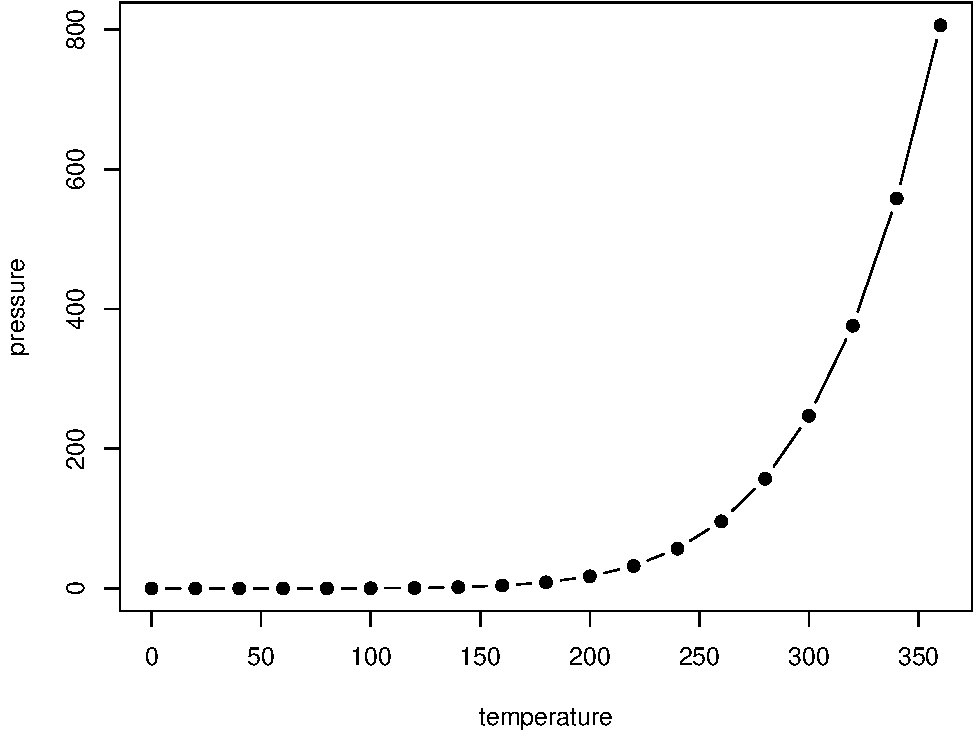
\includegraphics[width=0.8\linewidth]{_main_files/figure-latex/nice-fig-1} 

}

\caption{Here is a nice figure!}\label{fig:nice-fig}
\end{figure}

Don't miss Table \ref{tab:nice-tab}.

\begin{Shaded}
\begin{Highlighting}[]
\NormalTok{knitr}\SpecialCharTok{::}\FunctionTok{kable}\NormalTok{(}
  \FunctionTok{head}\NormalTok{(pressure, }\DecValTok{10}\NormalTok{), }\AttributeTok{caption =} \StringTok{\textquotesingle{}Here is a nice table!\textquotesingle{}}\NormalTok{,}
  \AttributeTok{booktabs =} \ConstantTok{TRUE}
\NormalTok{)}
\end{Highlighting}
\end{Shaded}

\begin{table}

\caption{\label{tab:nice-tab}Here is a nice table!}
\centering
\begin{tabular}[t]{rr}
\toprule
temperature & pressure\\
\midrule
0 & 0.0002\\
20 & 0.0012\\
40 & 0.0060\\
60 & 0.0300\\
80 & 0.0900\\
\addlinespace
100 & 0.2700\\
120 & 0.7500\\
140 & 1.8500\\
160 & 4.2000\\
180 & 8.8000\\
\bottomrule
\end{tabular}
\end{table}

You can add parts to organize one or more book chapters together. Parts can be inserted at the top of an .Rmd file, before the first-level chapter heading in that same file.

Add a numbered part: \texttt{\#\ (PART)\ Act\ one\ \{-\}} (followed by \texttt{\#\ A\ chapter})

Add an unnumbered part: \texttt{\#\ (PART\textbackslash{}*)\ Act\ one\ \{-\}} (followed by \texttt{\#\ A\ chapter})

Add an appendix as a special kind of un-numbered part: \texttt{\#\ (APPENDIX)\ Other\ stuff\ \{-\}} (followed by \texttt{\#\ A\ chapter}). Chapters in an appendix are prepended with letters instead of numbers.

\hypertarget{footnotes-and-citations}{%
\chapter{Footnotes and citations}\label{footnotes-and-citations}}

\hypertarget{footnotes}{%
\section{Footnotes}\label{footnotes}}

Footnotes are put inside the square brackets after a caret \texttt{\^{}{[}{]}}. Like this one \footnote{This is a footnote.}.

\hypertarget{citations}{%
\section{Citations}\label{citations}}

Reference items in your bibliography file(s) using \texttt{@key}.

For example, we are using the \textbf{bookdown} package \citep{R-bookdown} (check out the last code chunk in index.Rmd to see how this citation key was added) in this sample book, which was built on top of R Markdown and \textbf{knitr} \citep{xie2015} (this citation was added manually in an external file book.bib).
Note that the \texttt{.bib} files need to be listed in the index.Rmd with the YAML \texttt{bibliography} key.

The RStudio Visual Markdown Editor can also make it easier to insert citations: \url{https://rstudio.github.io/visual-markdown-editing/\#/citations}

\hypertarget{blocks}{%
\chapter{Blocks}\label{blocks}}

\hypertarget{equations}{%
\section{Equations}\label{equations}}

Here is an equation.

\begin{equation} 
  f\left(k\right) = \binom{n}{k} p^k\left(1-p\right)^{n-k}
  \label{eq:binom}
\end{equation}

You may refer to using \texttt{\textbackslash{}@ref(eq:binom)}, like see Equation \eqref{eq:binom}.

\hypertarget{theorems-and-proofs}{%
\section{Theorems and proofs}\label{theorems-and-proofs}}

Labeled theorems can be referenced in text using \texttt{\textbackslash{}@ref(thm:tri)}, for example, check out this smart theorem \ref{thm:tri}.

\begin{theorem}
\protect\hypertarget{thm:tri}{}\label{thm:tri}For a right triangle, if \(c\) denotes the \emph{length} of the hypotenuse
and \(a\) and \(b\) denote the lengths of the \textbf{other} two sides, we have
\[a^2 + b^2 = c^2\]
\end{theorem}

Read more here \url{https://bookdown.org/yihui/bookdown/markdown-extensions-by-bookdown.html}.

\hypertarget{callout-blocks}{%
\section{Callout blocks}\label{callout-blocks}}

The R Markdown Cookbook provides more help on how to use custom blocks to design your own callouts: \url{https://bookdown.org/yihui/rmarkdown-cookbook/custom-blocks.html}

\hypertarget{sharing-your-book}{%
\chapter{Sharing your book}\label{sharing-your-book}}

\hypertarget{publishing}{%
\section{Publishing}\label{publishing}}

HTML books can be published online, see: \url{https://bookdown.org/yihui/bookdown/publishing.html}

\hypertarget{pages}{%
\section{404 pages}\label{pages}}

By default, users will be directed to a 404 page if they try to access a webpage that cannot be found. If you'd like to customize your 404 page instead of using the default, you may add either a \texttt{\_404.Rmd} or \texttt{\_404.md} file to your project root and use code and/or Markdown syntax.

\hypertarget{metadata-for-sharing}{%
\section{Metadata for sharing}\label{metadata-for-sharing}}

Bookdown HTML books will provide HTML metadata for social sharing on platforms like Twitter, Facebook, and LinkedIn, using information you provide in the \texttt{index.Rmd} YAML. To setup, set the \texttt{url} for your book and the path to your \texttt{cover-image} file. Your book's \texttt{title} and \texttt{description} are also used.

This \texttt{gitbook} uses the same social sharing data across all chapters in your book- all links shared will look the same.

Specify your book's source repository on GitHub using the \texttt{edit} key under the configuration options in the \texttt{\_output.yml} file, which allows users to suggest an edit by linking to a chapter's source file.

Read more about the features of this output format here:

\url{https://pkgs.rstudio.com/bookdown/reference/gitbook.html}

Or use:

\begin{Shaded}
\begin{Highlighting}[]
\NormalTok{?bookdown}\SpecialCharTok{::}\NormalTok{gitbook}
\end{Highlighting}
\end{Shaded}

\hypertarget{useful-code}{%
\chapter{useful code}\label{useful-code}}

this is how you commit and push stuff in terminal
git add .

git commit -m ``commit message''

git push

ctrl + Alt + i = insert r script
echo = false means the scrubs dont see code

library(tidyr)
library(ggplot2)
library(readr)
library(dplyr)
library(tidyverse)
library(lubridate)

df1 \textless- read\_delim(``\_book/dailyMinTemp.csv'', delim = ``\textbar{}'')

data \textless- df1

data\_long \textless- data \%\textgreater\%
pivot\_longer(cols = -c(\texttt{Water\ Year}, Day),
names\_to = ``Month'',
values\_to = ``Temperature'')

month\_order \textless- c(``Jan'', ``Feb'', ``Mar'', ``Apr'', ``May'', ``Jun'', ``Jul'', ``Aug'', ``Sep'', ``Oct'', ``Nov'', ``Dec'')
data\_long \textless- data\_long \%\textgreater\%
mutate(
Month = factor(Month, levels = month\_order, ordered = TRUE),
Date = as.Date(paste(``2000'', Month, Day, sep = ``-''), format = ``\%Y-\%b-\%d'')
)

\hypertarget{calculate-the-average-temperature-for-each-day-across-all-years}{%
\chapter{Calculate the average temperature for each day across all years}\label{calculate-the-average-temperature-for-each-day-across-all-years}}

avg\_temp \textless- data\_long \%\textgreater\%
group\_by(Date) \%\textgreater\%
summarise(AvgTemperature = mean(Temperature, na.rm = TRUE))

\hypertarget{create-the-combined-line-graph}{%
\chapter{Create the combined line graph}\label{create-the-combined-line-graph}}

ggplot() +
\# Individual year lines
geom\_line(data = data\_long,
aes(x = Date, y = Temperature),
alpha = 0.5) +
\# Average temperature line
geom\_line(data = avg\_temp,
aes(x = Date, y = AvgTemperature),
color = ``black'', size = 1.2) +
scale\_x\_date(date\_labels = ``\%b'', date\_breaks = ``1 month'') +
scale\_color\_viridis\_d(option = ``plasma'') + \# Color-blind friendly palette
labs(title = ``Minimum Daily Temperature 2004-2024'',
x = ``Month'',
y = ``Temperature (Fahrenheit)'')
color = ``Water Year''

\begin{Shaded}
\begin{Highlighting}[]
\FunctionTok{library}\NormalTok{(plotly)}
\FunctionTok{library}\NormalTok{(tidyr)}
\FunctionTok{library}\NormalTok{(ggplot2)}
\FunctionTok{library}\NormalTok{(readr)}
\FunctionTok{library}\NormalTok{(dplyr)}
\FunctionTok{library}\NormalTok{(tidyverse)}
\FunctionTok{library}\NormalTok{(lubridate)}

\NormalTok{df1 }\OtherTok{\textless{}{-}} \FunctionTok{read\_delim}\NormalTok{(}\StringTok{"\_book/dailyAvgTemp.csv"}\NormalTok{, }\AttributeTok{delim =} \StringTok{"|"}\NormalTok{)}
\end{Highlighting}
\end{Shaded}

\begin{verbatim}
## Rows: 682 Columns: 14
## -- Column specification --------------------------------------------------------
## Delimiter: "|"
## dbl (14): Water Year, Day, Oct, Nov, Dec, Jan, Feb, Mar, Apr, May, Jun, Jul,...
## 
## i Use `spec()` to retrieve the full column specification for this data.
## i Specify the column types or set `show_col_types = FALSE` to quiet this message.
\end{verbatim}

\begin{Shaded}
\begin{Highlighting}[]
\NormalTok{data }\OtherTok{\textless{}{-}}\NormalTok{ df1}

\NormalTok{data\_long }\OtherTok{\textless{}{-}}\NormalTok{ data }\SpecialCharTok{\%\textgreater{}\%}
  \FunctionTok{pivot\_longer}\NormalTok{(}\AttributeTok{cols =} \SpecialCharTok{{-}}\FunctionTok{c}\NormalTok{(}\StringTok{\textasciigrave{}}\AttributeTok{Water Year}\StringTok{\textasciigrave{}}\NormalTok{, Day),}
               \AttributeTok{names\_to =} \StringTok{"Month"}\NormalTok{,}
               \AttributeTok{values\_to =} \StringTok{"Temperature"}\NormalTok{)}

\NormalTok{month\_order }\OtherTok{\textless{}{-}} \FunctionTok{c}\NormalTok{(}\StringTok{"Jan"}\NormalTok{, }\StringTok{"Feb"}\NormalTok{, }\StringTok{"Mar"}\NormalTok{, }\StringTok{"Apr"}\NormalTok{, }\StringTok{"May"}\NormalTok{, }\StringTok{"Jun"}\NormalTok{, }\StringTok{"Jul"}\NormalTok{, }\StringTok{"Aug"}\NormalTok{, }\StringTok{"Sep"}\NormalTok{, }\StringTok{"Oct"}\NormalTok{, }\StringTok{"Nov"}\NormalTok{, }\StringTok{"Dec"}\NormalTok{)}

\NormalTok{data\_long }\OtherTok{\textless{}{-}}\NormalTok{ data\_long }\SpecialCharTok{\%\textgreater{}\%}
  \FunctionTok{mutate}\NormalTok{(}
    \AttributeTok{Month =} \FunctionTok{factor}\NormalTok{(Month, }\AttributeTok{levels =}\NormalTok{ month\_order, }\AttributeTok{ordered =} \ConstantTok{TRUE}\NormalTok{),}
    \AttributeTok{Date =} \FunctionTok{as.Date}\NormalTok{(}\FunctionTok{paste}\NormalTok{(}\StringTok{"2000"}\NormalTok{, Month, Day, }\AttributeTok{sep =} \StringTok{"{-}"}\NormalTok{), }\AttributeTok{format =} \StringTok{"\%Y{-}\%b{-}\%d"}\NormalTok{),}
    \StringTok{\textasciigrave{}}\AttributeTok{Water Year}\StringTok{\textasciigrave{}} \OtherTok{=} \FunctionTok{as.factor}\NormalTok{(}\StringTok{\textasciigrave{}}\AttributeTok{Water Year}\StringTok{\textasciigrave{}}\NormalTok{),}
    \AttributeTok{hover\_text =} \FunctionTok{paste}\NormalTok{(}\StringTok{"Water Year:"}\NormalTok{, }\StringTok{\textasciigrave{}}\AttributeTok{Water Year}\StringTok{\textasciigrave{}}\NormalTok{, }\StringTok{"\textless{}br\textgreater{}"}\NormalTok{,}
                       \StringTok{"Month:"}\NormalTok{, Month, }\StringTok{"\textless{}br\textgreater{}"}\NormalTok{,}
                       \StringTok{"Day:"}\NormalTok{, Day, }\StringTok{"\textless{}br\textgreater{}"}\NormalTok{,}
                       \StringTok{"Temperature:"}\NormalTok{, }\FunctionTok{round}\NormalTok{(Temperature, }\DecValTok{1}\NormalTok{), }\StringTok{"°F"}\NormalTok{)}
\NormalTok{  ) }\SpecialCharTok{\%\textgreater{}\%}
  \FunctionTok{arrange}\NormalTok{(Month, Day)}

\CommentTok{\# Calculate the average temperature for each day of the year}
\NormalTok{avg\_temp }\OtherTok{\textless{}{-}}\NormalTok{ data\_long }\SpecialCharTok{\%\textgreater{}\%}
  \FunctionTok{group\_by}\NormalTok{(Month, Day) }\SpecialCharTok{\%\textgreater{}\%}
  \FunctionTok{summarise}\NormalTok{(}\AttributeTok{AvgTemperature =} \FunctionTok{mean}\NormalTok{(Temperature, }\AttributeTok{na.rm =} \ConstantTok{TRUE}\NormalTok{), }\AttributeTok{.groups =} \StringTok{\textquotesingle{}drop\textquotesingle{}}\NormalTok{) }\SpecialCharTok{\%\textgreater{}\%}
  \FunctionTok{mutate}\NormalTok{(}
    \AttributeTok{Date =} \FunctionTok{as.Date}\NormalTok{(}\FunctionTok{paste}\NormalTok{(}\StringTok{"2000"}\NormalTok{, Month, Day, }\AttributeTok{sep =} \StringTok{"{-}"}\NormalTok{), }\AttributeTok{format =} \StringTok{"\%Y{-}\%b{-}\%d"}\NormalTok{),}
    \AttributeTok{hover\_text =} \FunctionTok{paste}\NormalTok{(}\StringTok{"Average Temperature"}\NormalTok{, }\StringTok{"\textless{}br\textgreater{}"}\NormalTok{,}
                       \StringTok{"Month:"}\NormalTok{, Month, }\StringTok{"\textless{}br\textgreater{}"}\NormalTok{,}
                       \StringTok{"Day:"}\NormalTok{, Day, }\StringTok{"\textless{}br\textgreater{}"}\NormalTok{,}
                       \StringTok{"Temperature:"}\NormalTok{, }\FunctionTok{round}\NormalTok{(AvgTemperature, }\DecValTok{1}\NormalTok{), }\StringTok{"°F"}\NormalTok{)}
\NormalTok{  )}

\CommentTok{\# Create the combined line graph}
\NormalTok{p }\OtherTok{\textless{}{-}} \FunctionTok{ggplot}\NormalTok{() }\SpecialCharTok{+}
  \CommentTok{\# Individual year lines}
  \FunctionTok{geom\_line}\NormalTok{(}\AttributeTok{data =}\NormalTok{ data\_long, }
            \FunctionTok{aes}\NormalTok{(}\AttributeTok{x =}\NormalTok{ Date, }\AttributeTok{y =}\NormalTok{ Temperature, }\AttributeTok{color =} \StringTok{\textasciigrave{}}\AttributeTok{Water Year}\StringTok{\textasciigrave{}}\NormalTok{, }\AttributeTok{group =} \StringTok{\textasciigrave{}}\AttributeTok{Water Year}\StringTok{\textasciigrave{}}\NormalTok{, }\AttributeTok{text =}\NormalTok{ hover\_text), }
            \AttributeTok{alpha =} \FloatTok{0.5}\NormalTok{) }\SpecialCharTok{+}
  \CommentTok{\# Average temperature line}
  \FunctionTok{geom\_line}\NormalTok{(}\AttributeTok{data =}\NormalTok{ avg\_temp, }
            \FunctionTok{aes}\NormalTok{(}\AttributeTok{x =}\NormalTok{ Date, }\AttributeTok{y =}\NormalTok{ AvgTemperature),}
            \AttributeTok{color =} \StringTok{"black"}\NormalTok{, }\AttributeTok{size =} \FloatTok{1.2}\NormalTok{) }\SpecialCharTok{+}
  \FunctionTok{scale\_x\_date}\NormalTok{(}\AttributeTok{date\_labels =} \StringTok{"\%b"}\NormalTok{, }\AttributeTok{date\_breaks =} \StringTok{"1 month"}\NormalTok{) }\SpecialCharTok{+}
  \FunctionTok{scale\_color\_viridis\_d}\NormalTok{(}\AttributeTok{option =} \StringTok{"plasma"}\NormalTok{) }\SpecialCharTok{+}  \CommentTok{\# Color{-}blind friendly palette}
  \FunctionTok{labs}\NormalTok{(}\AttributeTok{title =} \StringTok{"Average Daily Temperature 2004{-}2024"}\NormalTok{,}
       \AttributeTok{x =} \StringTok{"Month"}\NormalTok{,}
       \AttributeTok{y =} \StringTok{"Temperature (Fahrenheit)"}\NormalTok{,}
       \AttributeTok{color =} \StringTok{"Water Year"}\NormalTok{) }\SpecialCharTok{+}
  \FunctionTok{theme\_minimal}\NormalTok{() }\SpecialCharTok{+}
  \FunctionTok{theme}\NormalTok{(}\AttributeTok{legend.position =} \StringTok{"right"}\NormalTok{,}
        \AttributeTok{axis.text.x =} \FunctionTok{element\_text}\NormalTok{(}\AttributeTok{angle =} \DecValTok{45}\NormalTok{, }\AttributeTok{hjust =} \DecValTok{1}\NormalTok{))}
\end{Highlighting}
\end{Shaded}

\begin{verbatim}
## Warning in geom_line(data = data_long, aes(x = Date, y = Temperature, color =
## `Water Year`, : Ignoring unknown aesthetics: text
\end{verbatim}

\begin{Shaded}
\begin{Highlighting}[]
\CommentTok{\# Convert to interactive plotly object with custom hover}
\NormalTok{p\_interactive }\OtherTok{\textless{}{-}} \FunctionTok{ggplotly}\NormalTok{(p, }\AttributeTok{tooltip =} \StringTok{"text"}\NormalTok{)}

\CommentTok{\# Modify hover template and mode}
\ControlFlowTok{for}\NormalTok{ (i }\ControlFlowTok{in} \DecValTok{1}\SpecialCharTok{:}\FunctionTok{length}\NormalTok{(p\_interactive}\SpecialCharTok{$}\NormalTok{x}\SpecialCharTok{$}\NormalTok{data)) \{}
\NormalTok{  p\_interactive}\SpecialCharTok{$}\NormalTok{x}\SpecialCharTok{$}\NormalTok{data[[i]]}\SpecialCharTok{$}\NormalTok{hoverinfo }\OtherTok{\textless{}{-}} \StringTok{"text"}
\NormalTok{  p\_interactive}\SpecialCharTok{$}\NormalTok{x}\SpecialCharTok{$}\NormalTok{data[[i]]}\SpecialCharTok{$}\NormalTok{hoverlabel }\OtherTok{\textless{}{-}} \FunctionTok{list}\NormalTok{(}\AttributeTok{bgcolor =} \StringTok{"white"}\NormalTok{)}
\NormalTok{\}}

\NormalTok{p\_interactive }\OtherTok{\textless{}{-}}\NormalTok{ p\_interactive }\SpecialCharTok{\%\textgreater{}\%} 
  \FunctionTok{layout}\NormalTok{(}\AttributeTok{hovermode =} \StringTok{"closest"}\NormalTok{)}

\CommentTok{\# Display the plot}
\NormalTok{p\_interactive}
\end{Highlighting}
\end{Shaded}

library(tidyr)
library(ggplot2)
library(readr)
library(dplyr)
library(tidyverse)
library(lubridate)
library(viridis)
library(plotly)

df1 \textless- read\_delim(``\_book/dailyPrecip.csv'', delim = ``\textbar{}'')

data \textless- df1 \%\textgreater\%
rename(Year = ``Water Year'')

data\_long \textless- data \%\textgreater\%
pivot\_longer(cols = -c(Year, Day),
names\_to = ``Month'',
values\_to = ``Precip'')

data\_long \textless- data\_long \%\textgreater\%
mutate(
MonthNum = match(Month, month.abb),
Date = make\_date(Year, MonthNum, Day),
MonthNum = NULL
) \%\textgreater\%
mutate(Date = ymd(Date))

\hypertarget{create-a-function-to-reorder-months-from-oct-to-sep}{%
\chapter{Create a function to reorder months from Oct to Sep}\label{create-a-function-to-reorder-months-from-oct-to-sep}}

reorder\_month \textless- function(x) \{
factor(x, levels = c(``Oct'', ``Nov'', ``Dec'', ``Jan'', ``Feb'', ``Mar'', ``Apr'', ``May'', ``Jun'', ``Jul'', ``Aug'', ``Sep''))
\}

\hypertarget{prepare-the-data-for-plotting}{%
\chapter{Prepare the data for plotting}\label{prepare-the-data-for-plotting}}

data\_plot \textless- data\_long \%\textgreater\%
mutate(
WaterYear = ifelse(month(Date) \textgreater= 10, Year, Year - 1),
Month = reorder\_month(Month)
) \%\textgreater\%
filter(Day == days\_in\_month(Date)) \%\textgreater\%
arrange(WaterYear, Month)

\hypertarget{calculate-average-cumulative-precipitation}{%
\chapter{Calculate average cumulative precipitation}\label{calculate-average-cumulative-precipitation}}

avg\_precip \textless- data\_plot \%\textgreater\%
group\_by(Month) \%\textgreater\%
summarize(AvgPrecip = mean(Precip, na.rm = TRUE))

data\_plot\(WaterYear <- as.factor(data_plot\)WaterYear)

\hypertarget{create-the-plot}{%
\chapter{Create the plot}\label{create-the-plot}}

p \textless- ggplot() +
geom\_line(data = data\_plot, aes(x = Month, y = Precip, group = WaterYear, color = WaterYear),
linewidth = 1) +
geom\_line(data = avg\_precip, aes(x = Month, y = AvgPrecip, group = 1),
linewidth = 1.5, color = ``black'') +
geom\_point(data = avg\_precip, aes(x = Month, y = AvgPrecip),
size = 1, color = ``black'') +
scale\_x\_discrete(limits = levels(reorder\_month(avg\_precip\$Month))) +
scale\_color\_viridis(discrete = TRUE, option = ``plasma'', name = ``Water Year'') +
labs(
title = ``Average Cumulative Precipitation 2004-2024'',
x = ``Month'',
y = ``Cumulative Precipitation (Inches)''
) +
theme\_minimal() +
theme(
legend.position = ``right'',
axis.text.x = element\_text(angle = 45, hjust = 1),
panel.grid.minor = element\_blank(),
legend.key = element\_rect(fill = ``white'', colour = NA),
legend.key.size = unit(0.8, ``cm'')
)

plotly\_plot \textless- ggplotly(p)

  \bibliography{book.bib,packages.bib}

\end{document}
